\newgeometry{margin=1.5cm}

\pagestyle{empty}

%\lhead{ 
\begin{tabular}{p{15cm}p{5cm}}
  
\includegraphics{0_frontmatter/figures/LogoEII.jpg}   &  TFT04\\
\end{tabular}
%}

\vspace{1em}
\fboxrule=2pt
\begin{center}
\fcolorbox{gray}{gray!10}{\parbox{.65\textwidth}{ {\large SOLICITUD DE DEFENSA DE TRABAJO DE FIN DE TÍTULO}}}
\end{center}

\vspace{1em}
\justify
D./Dª \underline{Prashant Jeswani Tejwani}, autor del Trabajo de Fin de Título \underline{Clasificador mediante imágenes de}

\underline{cáncer de piel}, correspondiente a la titulación Grado de Ingeniería Informática.

\vspace{1em}
SOLICITA

\vspace{1em}
que se inicie el procedimiento de defensa del mismo, para lo que se adjunta la documentación requerida, haciendo constar que 
\vspace{1em}

\hspace{10mm} [X] se autoriza / [ ] no se autoriza la grabación en audio de la exposición y turno de preguntas.

\vspace{1em}
Asimismo, con respecto al registro de la propiedad intelectual/industrial del TFT, declara que:
\vspace{1em}

\hspace{10mm} [ ] Se ha iniciado o hay intención de iniciarlo (defensa no pública).

\hspace{10mm} [X] No está previsto.

\vspace{1em}
Y para que así conste firma la presente. 

\begin{center}
En Las Palmas de Gran Canaria, a 26 de octubre de 2021

\vspace{1em}
El estudiante

\vspace{3em}
Fdo.------------------------
\end{center}

\begin{center}

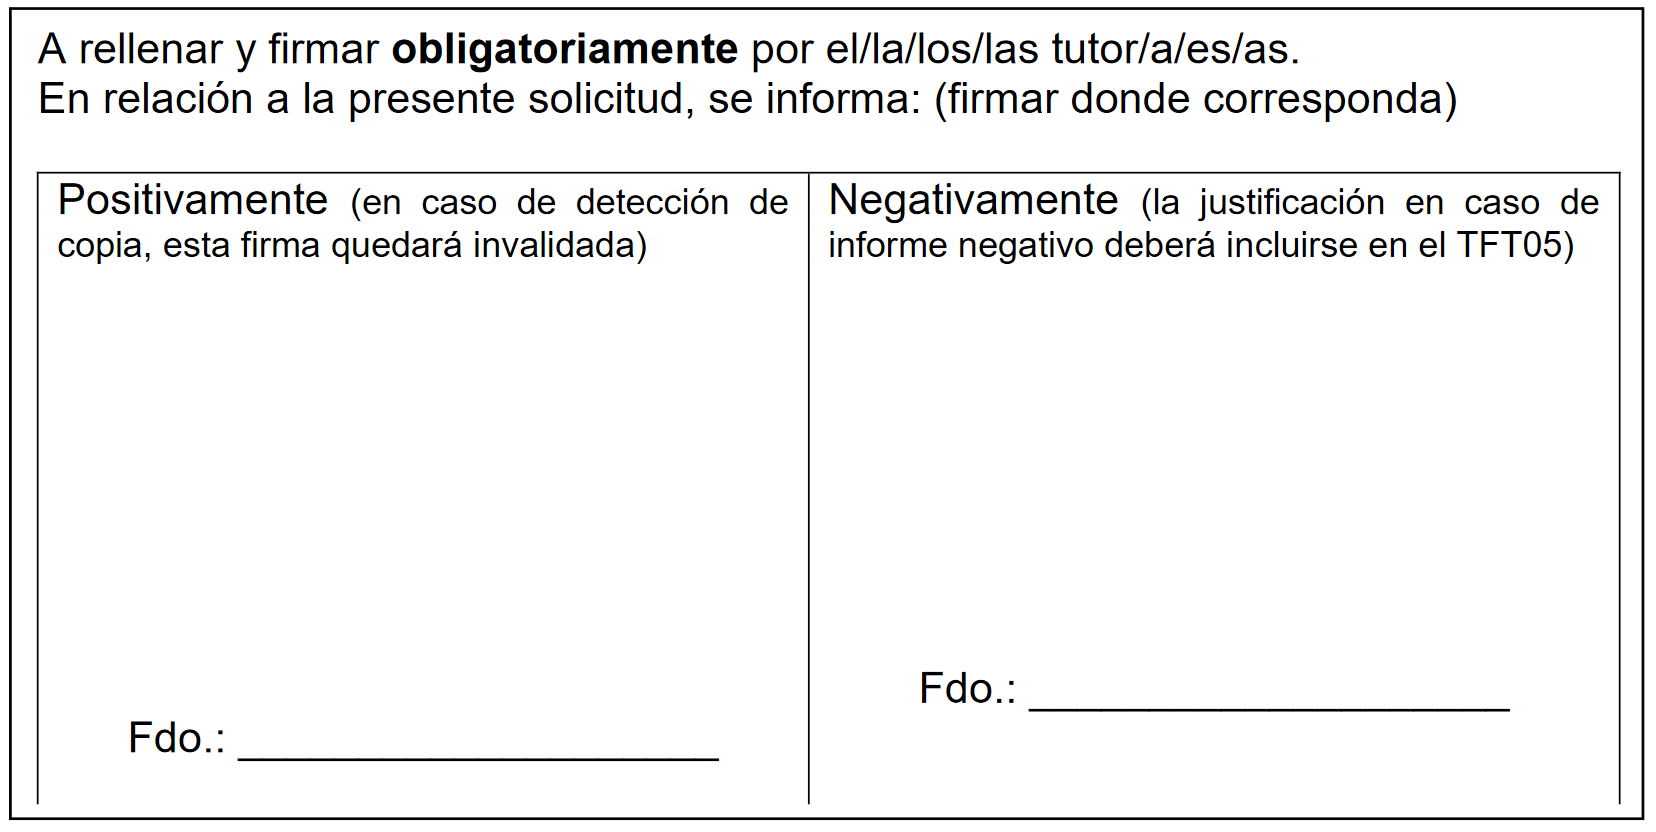
\includegraphics[scale=0.6]{0_frontmatter/figures/firmasTFT04.PNG}

%\fcolorbox{gray}{white!10}{\parbox{.75\textwidth}{
%A rellenar y firmar \textbf{obligatoriamente} por %el/la/los/las tutor/a/es/as.

%En relación con la presente solicitud, se informa:

%\vspace{1em}
%\begin{tabular}{lr}
  %[X] Positivamente  & [ ] Negativamente (justificación %en TFT05)\\
%\end{tabular} 

%\vspace{3em}
%\center{Fdo.------------------------ }
%
%}}

\vspace{1em}

%\cfoot{
DIRECTOR DE LA ESCUELA DE INGENIERÍA INFORMÁTICA
%}

\end{center}

\restoregeometry